\section{Results}
\label{sec:results}

We organize results around two questions. Does the regularizer improve retrieval accuracy across language pairs (Section~\ref{sec:results-retrieval})? Does it reshape token geometry as designed (Section~\ref{sec:results-geometry})?

\begin{table}[t]
\centering
\caption{Cross-lingual retrieval accuracy on FLORES+. Numbers are MaxSim P@1 mean $\pm$ standard deviation across 3 seeds. EN-ES is the language pair used for training; all others are zero-shot. Effect-size markers (not statistical significance) compare IsoColBERT to vanilla, computed against the larger of the two seed-wise standard deviations: \textbf{***}~$\Delta\mu > 2\sigma$, \textbf{**}~$\Delta\mu > \sigma$, \textbf{*}~$\Delta\mu > \sigma/2$.}
\label{tab:retrieval}
\small
\begin{tabular}{lcc}
\toprule
Language pair & Vanilla & IsoColBERT ($\lambda{=}0.5$) \\
\midrule
EN--ES (seen)    & $0.9973 \pm 0.0010$ & $0.9968 \pm 0.0002$ \\
EN--FR           & $0.9983 \pm 0.0006$ & $0.9988 \pm 0.0002$\textsuperscript{*} \\
EN--DE           & $0.9957 \pm 0.0006$ & $\mathbf{0.9978 \pm 0.0013}$\textsuperscript{**} \\
EN--SW           & $0.8344 \pm 0.0230$ & $\mathbf{0.8689 \pm 0.0227}$\textsuperscript{**} \\
EN--AR           & $0.9423 \pm 0.0204$ & $\mathbf{0.9622 \pm 0.0132}$\textsuperscript{*} \\
EN--NE           & $0.9008 \pm 0.0176$ & $\mathbf{0.9154 \pm 0.0106}$\textsuperscript{*} \\
EN--TA           & $0.9066 \pm 0.0133$ & $0.9154 \pm 0.0192$ \\
\bottomrule
\end{tabular}
\end{table}

\begin{figure}[t]
\centering
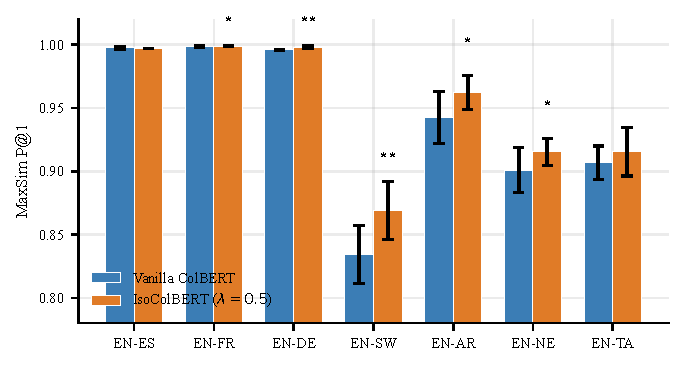
\includegraphics[width=\columnwidth]{figs/fig_main_p1.pdf}
\caption{MaxSim P@1 across seven language pairs, vanilla vs.\ IsoColBERT ($\lambda{=}0.5$), 3-seed mean with $\pm$ standard deviation error bars. Effect-size markers (not statistical significance) compare to vanilla. High-resource pairs are at retrieval ceiling for both methods; the four low-resource pairs (SW, AR, NE, TA) show consistent positive deltas in the mean.}
\label{fig:retrieval}
\end{figure}

\begin{figure}[t]
\centering
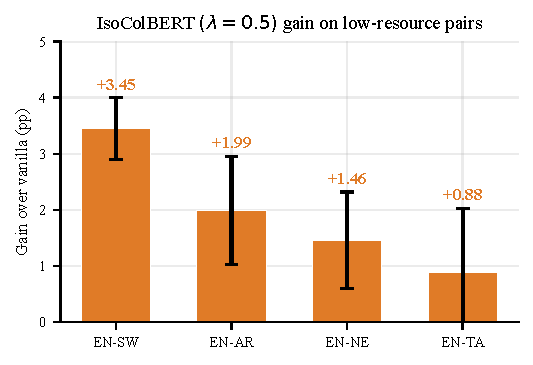
\includegraphics[width=\columnwidth]{figs/fig_low_resource_gains.pdf}
\caption{Pp gain of IsoColBERT over vanilla on the four low-resource pairs (3-seed mean $\pm$ seed-wise std of the gain). The high-resource pairs are saturated in Figure~\ref{fig:retrieval}; this view isolates the regime where the gains live and shows the resource-ordering pattern: the largest gain is on Swahili (lowest pretraining resource), the smallest on Tamil (most pretraining resource among the four).}
\label{fig:retrieval-low}
\end{figure}

\subsection{Retrieval Accuracy}
\label{sec:results-retrieval}

Table~\ref{tab:retrieval} reports MaxSim P@1 across the seven FLORES+ language pairs. On English-Swahili, IsoColBERT improves P@1 from $0.8344 \pm 0.0230$ to $0.8689 \pm 0.0227$, a gain of $3.45$ percentage points; the EN-AR gain is $1.99$ percentage points (from $0.9423$ to $0.9622$). The gains extend zero-shot to Nepali ($+1.46$ pp) and Tamil ($+0.88$ pp), two further low-resource languages that the model never saw during training. The three high-resource pairs (EN-ES, EN-FR, EN-DE) sit at $0.996$ P@1 or above for both methods, with differences within one standard deviation. EN-ES is the only pair on which the model is trained; the other six are evaluated zero-shot, so the low-resource gains transfer through XLM-R's shared multilingual encoder without any in-language supervision. Figure~\ref{fig:retrieval} visualizes the absolute P@1 comparison; Figure~\ref{fig:retrieval-low} zooms in on the four low-resource pairs as pp gain over vanilla, which is where the effect is visible.

\paragraph{Per-seed consistency.} The EN-SW gain is positive on every seed individually: $+3.09$, $+4.08$, and $+3.19$ percentage points on seeds $42$, $1337$, and $2024$ respectively. EN-AR and EN-NE are likewise positive on every seed (EN-AR: $+1.79$, $+1.14$, $+3.04$; EN-NE: $+0.69$, $+1.30$, $+2.39$). EN-TA improves on two of three seeds (with seed $2024$ showing a $-0.45$ pp shift), reflecting the smaller average effect on this pair. The regularizer's seed-wise standard deviation on EN-SW is essentially unchanged from vanilla ($0.0230 \to 0.0227$): the gain is added to a noisy baseline rather than coming from variance reduction.

\paragraph{Where the gains concentrate.} The pattern in Table~\ref{tab:retrieval} is interpretable as the intersection of two conditions: pretrained-signal scarcity and retrieval headroom. High-resource pairs sit at the ceiling because XLM-R was pretrained on far more Spanish, French, and German text than any of the low-resource four, leaving no room for either method to improve. The four low-resource pairs all have weak pretrained signal and room to grow on retrieval, and the largest gain is on the lowest-resource language. Swahili (roughly $1.6$\,GB of pretraining text per \citet{conneau2020xlmr}) sits at the bottom and shows the largest gain ($+3.45$ pp); Arabic ($+1.99$ pp), Nepali ($+1.46$ pp), and Tamil ($+0.88$ pp) follow. The ordering of the latter three is not strictly monotonic in XLM-R pretraining-data size --- Arabic has substantially more pretraining text ($\approx 28$\,GB) than Nepali ($\approx 2.4$\,GB) or Tamil ($\approx 12$\,GB) but a larger gain. Pretrained-signal scarcity is therefore one factor driving the gain pattern, but per-language properties such as script and morphology likely also shape the available retrieval headroom.

\subsection{Token Geometry}
\label{sec:results-geometry}

Table~\ref{tab:geometry} and Figure~\ref{fig:geometry} report the intra-cosine similarity and effective rank of token vectors before and after applying IsoColBERT, for English and Spanish tokens drawn from the FLORES+ dev set. Both metrics move in the direction the regularizer was designed to push them. Intra-cosine drops from $0.20$ to $0.17$ on English and from $0.29$ to $0.18$ on Spanish. Effective rank rises from $105.1$ to $107.5$ on English and from $101.7$ to $106.7$ on Spanish. All four geometric shifts have $\Delta\mu > 2\sigma$ relative to the IsoColBERT seed-wise standard deviation and are consistent in sign across all three seeds.

\begin{table}[t]
\centering
\caption{Token-level geometry on FLORES+ valid token vectors. Intra-cosine is mean off-diagonal cosine over 2048 tokens per language (lower is more isotropic). Effective rank is computed over 4096 tokens per language (higher is more isotropic). Numbers are 3-seed means.}
\label{tab:geometry}
\small
\begin{tabular}{lcccc}
\toprule
 & \multicolumn{2}{c}{Intra-cos $\downarrow$} & \multicolumn{2}{c}{eRank $\uparrow$} \\
\cmidrule(lr){2-3} \cmidrule(lr){4-5}
Method & EN & ES & EN & ES \\
\midrule
Vanilla        & $0.2015$ & $0.2937$ & $105.06$ & $101.73$ \\
IsoColBERT     & $\mathbf{0.1718}$ & $\mathbf{0.1808}$ & $\mathbf{107.50}$ & $\mathbf{106.70}$ \\
$\Delta$       & $-0.030$ & $-0.113$ & $+2.44$ & $+4.98$ \\
\bottomrule
\end{tabular}
\end{table}

\begin{figure*}[t]
\centering
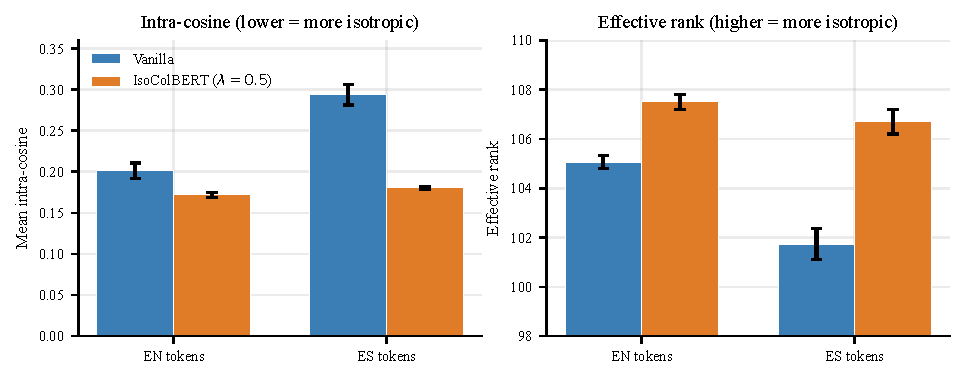
\includegraphics[width=\textwidth]{figs/fig_geometric.pdf}
\caption{Token-level geometry shifts toward isotropy under IsoColBERT. Intra-cosine (left, lower = more isotropic) drops on both languages, with the larger shift on Spanish. Effective rank (right, higher = more isotropic) rises on both languages, again with the larger shift on Spanish. 3-seed mean with $\pm$ standard deviation error bars.}
\label{fig:geometry}
\end{figure*}

\paragraph{Asymmetric collapse and asymmetric recovery.} A consistent pattern across both metrics is that Spanish tokens are more anisotropic than English tokens under vanilla training and more strongly reshaped under IsoColBERT. The vanilla intra-cosine gap is $0.094$ in favor of English ($0.29$ on ES vs.\ $0.20$ on EN); the IsoColBERT gap closes to $0.009$. The effective rank gap closes similarly: $3.33$ down to $0.80$. We attribute the asymmetry to the structure of bitext InfoNCE. The loss in \eqref{eq:infonce} is symmetric in source and target, but the encoder is pretrained on far more English text than Spanish text. Under contrastive pressure, the Spanish-side representations have more to learn and bear most of the gradient signal, which is precisely the regime where the embedding manifold collapses hardest. IsoColBERT redistributes that gradient: instead of letting target-side representations contract into a narrow cone, the regularizer maintains angular separation. This is consistent with the observation that the four low-resource targets — and Swahili in particular — gain the most retrieval accuracy.

\paragraph{Geometry tracks retrieval.} The four geometric metrics (EN/ES intra-cosine, EN/ES effective rank) all clear the \textbf{***} effect-size cutoff ($\Delta\mu > 2\sigma$) with all three seeds positive, and the retrieval gains on the four low-resource pairs (EN-SW, EN-AR, EN-NE, EN-TA) are positive in the mean and on at least two of three seeds in every case. Because the loss in \eqref{eq:loss} explicitly optimizes geometry, this co-movement is correlational rather than causal. We cannot rule out, in particular, that the regularizer also (a) acts as general capacity regularization by penalizing overconfident or high-norm token representations and so improves accuracy through the standard regularization channel; (b) reshapes optimization dynamics indirectly (for example by smoothing the contrastive loss surface) in a way that helps the low-resource pairs disproportionately; or (c) affects cross-lingual alignment through paths that do not pass through token-level intra-cosine and effective rank. What we can say is that geometric reshaping is the only quantity the regularizer directly targets, and that the gain pattern (concentrated on low-resource targets, scaling with vanilla anisotropy) is consistent with the predicted mechanism. Mechanism ablations (Section~\ref{sec:ablations-mechanism}) further constrain the candidates: of the three regularizer placements we tested, only the one that reshapes the full token manifold recovers the retrieval gain.

